%-------------------------------------------------------------------------------
% event_editor
%-------------------------------------------------------------------------------
%
% \file        event_editor.tex
% \library     Documents
% \author      Chris Ahlstrom
% \date        2016-01-02
% \update      2023-09-20
% \version     $Revision$
% \license     $XPC_GPL_LICENSE$
%
%-------------------------------------------------------------------------------

\section{Event Editor}
\label{sec:event_editor}

   The \textsl{Seq66} \textbf{Event Editor} tab is used to view and edit,
   in detail, the events present in a loop / sequence / pattern / track.
   It is accessed by right-clicking on a pattern in the \textbf{Live} frame,
   then selecting the \textbf{Edit pattern in tab} menu entry.
   The default keystroke combination for this action is to use the minus key
   followed by the desired pattern's hot-key.

   The event editor is not very sophisticated.
   It is a basic editor for simple edits, viewing, and trouble-shooting.
   It is disabled if recording a pattern, to avoid refresh issues while
   recording.

   Viewing and scrolling work;
   editing, deleting, and inserting events work.
   But there are many possible interactions between event links
   (Note Off events linked to Note On events, for example),
   performance triggers, and the pattern,
   performance, and event editor dialogs.
   Surely some bugs still lurk.
   If anything bad happens, do \textsl{not} press the
   \textbf{Save to Sequence} button!
   If the application aborts, let us know!
   Here are the major "issues":

   \begin{enumerate}
      \item It requires the user to know the details
         about MIDI events and data values.
      \item For safety, it does not detect any changes made to the sequence in
         the pattern editor; we might add a refresh button.
      \item It does not have an undo function.
      \item It cannot mark more than one event for deletion or modification.
         However, if one note event is deleted, the corrsponding linked note
         event is also deleted.
      \item There is no support for dragging and dropping of events.
   \end{enumerate}

   The event editor is a good way to see the events in a sequence,
   and to delete or modify problematic events.
   Additionally, it can be used to add \textbf{Set Tempo} and other
   meta events.
   \index{sequence extension}
   \index{pattern extension}
   If an event is added that has a time-stamp beyond the current
   length of the sequence, then the length of the sequence is extended.
   Unlike the event pane in the pattern editor, the event-editor
   dialog shows all types of events at once.

\begin{figure}[H]
   \centering
   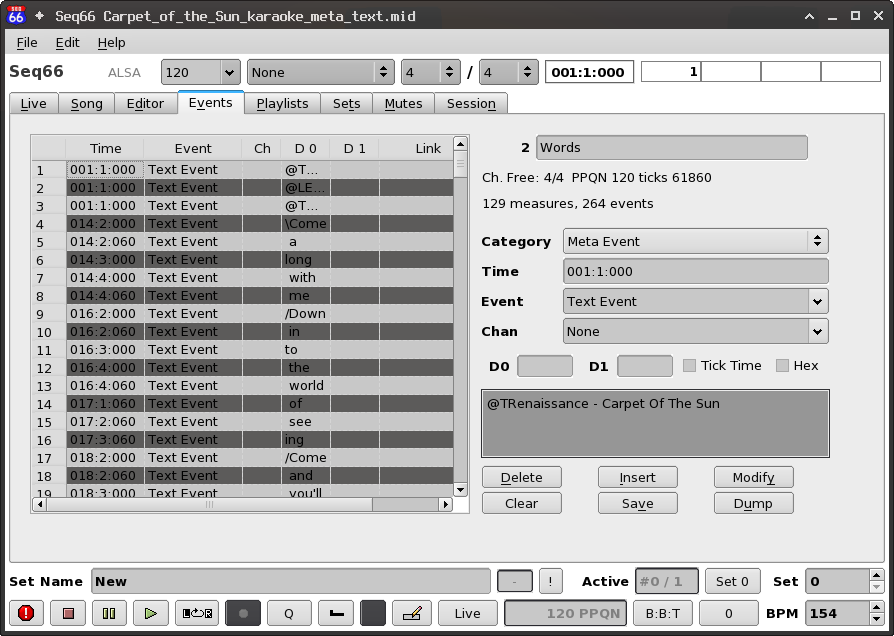
\includegraphics[scale=0.65]{event-editor/event-editor-tab.png}
   \caption{Event Editor Window}
   \label{fig:event_editor_window}
\end{figure}

   The event-editor dialog is fairly complex.
   For exposition, we break it down into a few sections:

   \begin{enumber}
      \item \textbf{Event Frame}
      \item \textbf{Info Panel}
      \item \textbf{Edit Fields}
      \item \textbf{Bottom Buttons}
   \end{enumber}

   The event frame is a list of events, which can be traversed, and edited.
   The fields in the right panel show the name of
   the pattern containing the events and other information about the
   pattern.  The edit fields provide text fields for viewing and entering
   information about the current event, and buttons to delete, insert, and
   modify events.  The bottom buttons allow changes to be saved and the editor
   to be closed.  
   The following sections described these items in detail.

\subsection{Event Editor / Event Frame}
\label{subsec:event_editor_frame}

   The event frame is the event-list shown on the left side of the
   event editor.  It is accompanied by a vertical scroll-bar, for moving one
   line or one page at a time.
   Mouse or touchpad scrolling can be used to move up and down
   in the event list.  This movement is even easier than reaching for the
   scrollbars.
   Depending on the window manager theme, the currently-selected event
   is highlighted.
   (We have been trying to get this table to auto-stretch vertically when the
   main window is vertically maximized, but have not succeeded so far. Qt!)

\subsubsection{Event Frame / Data Items}
\label{subsec:event_frame_data}

   The event frame shows a list of numbered events, one per line.
   The currently-selected event is shown in the edit fields.
   Here is an example of the data line for a MIDI event:

   \begin{verbatim}
      17   003:3:128 Note On   Ch 3    0x45:69 0x6b:107 003:4:96
   \end{verbatim}

   This line consists of the following parts:

   \begin{enumber}
      \item \textbf{Index Number}
      \item \textbf{Time Stamp}
      \item \textbf{Event Name}
      \item \textbf{Channel Number}
      \item \textbf{Data Bytes}
      \item \textbf{Link}
   \end{enumber}

   \setcounter{ItemCounter}{0}      % Reset the ItemCounter for this list.

   \itempar{Index Number}{event editor!index number}
   Displays the index number of the event.
   This number is purely for reference, and is not part
   of the event.  Events in the pattern are numbered from 1 to the number of
   events in the pattern.

   \itempar{Time Stamp}{event editor!time stamp}
   Displays the time stamp of the event,
   which indicates the cumulative time of the event in the pattern.
   It is displayed in the format of "measure:beat:divisions".
   The measure values start from 1, and range up to the number of measures in
   the pattern.
   The beat values start from 1, and range up to the number of beats in the
   measure.
   The division values range from 0 up to one less than the
   \index{ppqn}
   PPQN (pulses per quarter note) value for the whole song.
   \index{ppqn!\$ shortcut}
   As a shortcut, one can use the dollar sign ("\$") to represent
   PPQN-1.
   If the \textbf{Tick Time} box is checked, then the timestamps are
   shown in units of "ticks" (MIDI pulses, sometimes called "divisions").

   \itempar{Event Name}{event editor!event name}
   Displays the name of the event.
   The event name indicates what kind of MIDI event it is. 
   See \sectionref{subsec:event_editor_fields}.

   \itempar{Channel Number}{event editor!channel number}
   Shows the channel number (for channel-events only) re 1, not 0.
   (For the user, MIDI channels always range from
   1 to 16.  Internally, they range from 0 to 15.)

   \itempar{Data Bytes}{event editor!data bytes}
   Shows the one or two data bytes for the event.
   The byte is shown in two formats, hexadecimal and decimal, as in
   \texttt{0x6b:107} ("hex:dec").
   For text events, a small portion of the text is shown.

   Note Off, Note On, and Aftertouch events requires a byte for the key (0 to
   127) and a byte for the velocity (also 0 to 127).
   Control Change events require a control code and a value for that control
   code.  Pitch wheel events require two bytes to encode the full range of
   pitch changes.
   Program change events require only a byte value to pick the patch or program
   (instrument) to be used for the sequence.  The Channel Pressure event
   requires only a one-byte value.
   Tempo requires a number (e.g. "120.3") to be typed in.

   \itempar{Links}{event editor!links}
   Note events are linked together; each Note On is linked to the corresponding
   Note Off, and vice versa.

\subsubsection{Event Frame / Navigation}
\label{subsec:event_frame_navigation}

   Moving about in the event frame is straightforward, but has some
   wrinkles to note.
   Navigation with the mouse is done by moving to the desired event and
   clicking on it.  The event becomes highlighted, and its data items are shown
   in the "info panel".
   There is no support for dragging and dropping events in the event frame.
   There is no support for selecting multiple events.

   The scrollbar can be used to move within the frame, either by one line at a
   time, or by a page at a time.  A page is defined as one frame's worth of
   lines, minus 5 lines, for some overlap in paging.

   Navigation with keystrokes is also supported, for the Up and Down arrows and
   the Page-Up and Page-Down keys.  Note that using the Up and Down arrows by
   holding them down for awhile causes autorepeat to kick in.
   Use the scrollbar or page keys to
   move through multiple pages.  Home and End also work.

\subsection{Event Editor / Info Panel}
\label{subsec:event_editor_info}

   The "info panel" is a read-only list of properties on the top right
   of the event editor.  It serves to remind the used of the pattern being
   edited and some characteristics of the pattern and the whole song.
   It also includes one button.
   Five items are shown:

   \begin{enumber}
      \item \textbf{Sel Linked}. (Not yet shown)
         If this button is checked, then selecting a Note On or Off event
         also selects the opposite, linked note.
         This allow for easy deletion of a complete Note pair.
      \item \textbf{Sequence Number and Name}.
         A bit redundant, as the window caption or the pattern
         also shows the pattern name.
         It can be set here or in the pattern editor.
      \item \textbf{Time Signature}.
         A pattern property, shown only as a reminder.
         It can be set in the pattern editor.
      \item \textbf{PPQN}
         Shows the "parts per quarter note", or resolution of the
         whole song.  The default PPQN of \textsl{Seq66} is 192.
      \item \textbf{Sequence Channel}
         In \textsl{Seq66}, the channel number is a property of the
         pattern.  All channel events in the pattern get routed to the same
         channel, even if somehow the event itself specifies a different
         channel.
      \item \textbf{Sequence Count}
         Displays the current number of events in the pattern.
         This number changes as events are inserted or deleted.
   \end{enumber}

\subsection{Event Editor / Edit Fields}
\label{subsec:event_editor_fields}

   The edit fields show the values of the currently-selected event.  They allow
   changing an event, adding a new event, or deleting the currently-selected
   event.

   \begin{enumber}
      \item \textbf{Event Category} (bold-faced, read-only)
      \item \textbf{Time} (event timestamp)
      \item \textbf{Event} (event name)
      \item \textbf{D0} (data byte 1)
      \item \textbf{D1} (data byte 2)
      \item \textbf{Show data in hex format} (not shown in figure)
   \end{enumber}

   \textbf{Important}: changes made in the event editor
   are \textsl{not written} to the sequence until the \textbf{Save}
   button is clicked.  If one messes up an edit field, just click on the event
   again; all the fields will be filled in again.
   That's as much "undo" as the event-editor offers at this time, other than
   closing without saving.

   \setcounter{ItemCounter}{0}      % Reset the ItemCounter for this list.

   \itempar{Event Category}{event editor!event category}
   Displays the event category of the event in bold-face.
   Currently, only channel events
   and a couple of meta events,
   can be handled, but someday we hope to handle the wide array of system
   events, and perhap even system-exclusive events.

   \itempar{Time}{event editor!event timestamp}
   Displays the timestamp of the event.  Currently only the
   "measure:beat:division" format is fully supported.
   We allow editing (but not display) of the timestamp in
   pulse (divisions) format and "hour:minute:second.fraction" format, but
   there are bugs to work out.

   If one wants to delete or modify an event, this field does not need to be
   modified.  If this field is modified, and the \textbf{Modify}
   button is pressed, then the event will be moved.  This field can locate
   a new event at a specific time.  If the time is not in the current frame,
   the frame will move to the location of the new event and make it the current
   event.

   \itempar{Category}{event editor!event category}
   This drop-down displays the category of the currently selected event:

\begin{figure}[H]
   \centering
   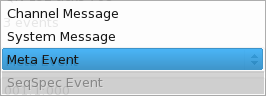
\includegraphics[scale=0.65]{event-editor/message-category-dropdown.png}
   \caption{Event Category List}
   \label{fig:event_editor_category_dropdown}
\end{figure}

   There are four types of messages handled by \textsl{Seq66}:
   Channel, System, Meta, and SeqSpec. 
   Seqspec messages are stored when a pattern is saved, but they are
   not part of the pattern's event list.
   Hence this item is grayed out; these message values are shown in various
   parts of the user interface.
   See the table in \sectionref{subsec:midi_format_meta_format}.

   \itempar{Time}{event editor!event time}
   Shows the time of the event in the format of "measure:beat:divisions" (only).
   This field can be edited to change the time of the event.

   \itempar{Event}{event editor!event name}
   Displays the name of the event, and allows entry of an event name.
   The event name indicates what kind of MIDI event it is. 
   The following event names are supported for Channel events:

   \begin{enumber}
      \item \textbf{Note Off}
      \item \textbf{Note On}
      \item \textbf{Aftertouch}
      \item \textbf{Control Change}
      \item \textbf{Program Change}
      \item \textbf{Channel Pressure}
      \item \textbf{Pitch Wheel}
      \item \textbf{Tempo}
   \end{enumber}

   Selecting one of these names from the dropdown changes the kind of event if
   the event is modified.  Abbreviations and case-insensitivity can be used to
   reduce the effort of typing.
   Also, if \textbf{Control Change} or
   \textbf{Program Change} are selected, then a data drop-down box is available
   to select either the controller or
   the instrument patch (program), and it can fill in the data values.
   In the future, we may make these configurable, with the control-change
   following the settings in the 'usr' file, and the program-change being made
   from a (new) 'patch' file. Currently the programs are General MIDI.

   If the \textbf{Meta Event} category is selected, the following events are
   shown:

\begin{figure}[H]
   \centering
   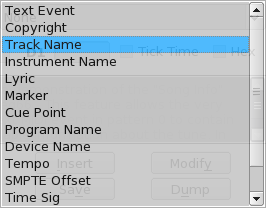
\includegraphics[scale=0.65]{event-editor/meta-event-dropdown.png}
   \caption{Meta Event List}
   \label{fig:event_editor_meta_dropdown}
\end{figure}

   If the \textbf{System Message} category is selected, the following events are
   shown:

\begin{figure}[H]
   \centering
   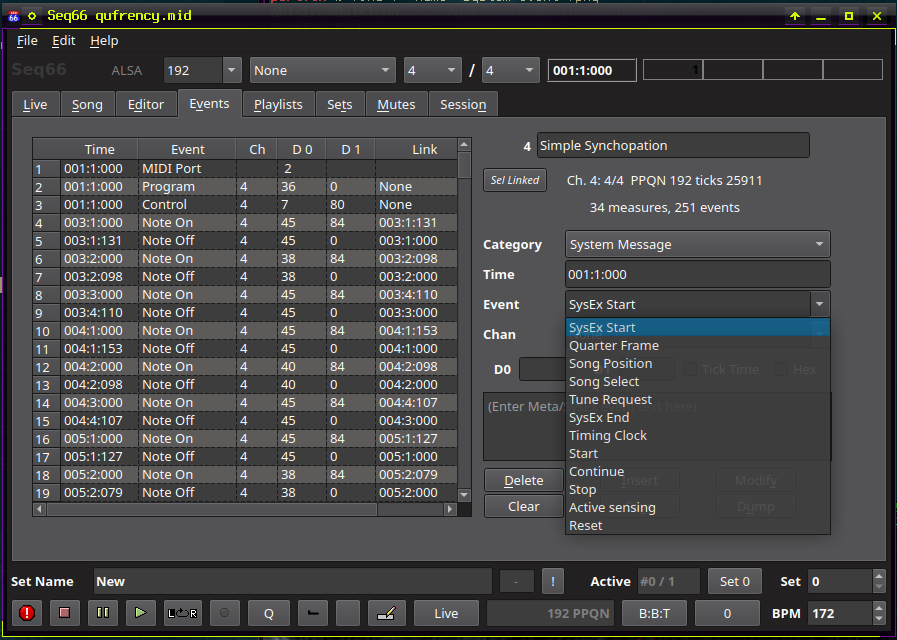
\includegraphics[scale=0.65]{event-editor/system-event-dropdown.png}
   \caption{System Message List}
   \label{fig:event_editor_system_dropdown}
\end{figure}

   At present, most of these message are not editable, but at least they can be
   seen.

   \itempar{Channel}{event editor!channel}
   This dropdown shows the channel of the current event, ranging from 1 to 16.
   If the event is not a channel message, then \textbf{None} is shown.

   \itempar{D0}{event editor!data byte 1}
   Allows modification of the first data byte of the event.
   One must know what one is doing.
   The scanning of the digits is very simple:  start with the first digit, and
   convert until a non-digit is encountered.  The data-byte value can be
   entered in decimal notation, or, if prepended with "0x", in hexadecimal
   notation.

   For a Tempo setting only this field is used; Data Byte 2 is ignored.
   Enter a Tempo value, such as "120", and then click \textbf{Insert}. The
   value is converted to the 3 bytes of a tempo event, and then
   added at the given timestamp.  (Screen refresh is not perfect yet, but
   reloading the pattern shows the correct tempo.)

   \itempar{D1}{event editor!data byte 2}
   Allows modification of the second data byte of the event (if applicable
   to the event).
   One must know what one is doing.
   The scanning of the digits is as noted above.

   \itempar{Tick time}{event editor!tick time}
   Selecting this check-box
   shows the time-stamps in the frame in tick (pulses) format.

   \itempar{Hex}{event editor!hex data}
   Selecting this check-box
   shows all number items in hex format.

   \itempar{Text data}{event editor!text data}
   This unlabelled pane shows the text of a meta text event.
   This field can be edited to add or change a meta text event.
   The events supported are:
   \textsl{Text Event},
   \textsl{Copyright},
   \textsl{Instrument Name},
   \textsl{Lyric},
   \textsl{Program Name}, and
   \textsl{Device Name}.

%  \itempar{Delete}{event editor!delete event}
%  Causes the selected event to be deleted.
%  The frame display is updated to move following events upward.

\subsection{Event Editor / Bottom Buttons}
\label{subsec:event_editor_buttons}

   These are the buttons that act on the edit fields or current event
   selection:

   \begin{enumber}
      \item \textbf{Delete} (selected event)
      \item \textbf{Insert} (new event)
      \item \textbf{Modify} (selected event)
      \item \textbf{Clear} (all events)
      \item \textbf{Save} (back to pattern)
      \item \textbf{Dump} (dump the events to a file)
   \end{enumber}

   Note that
   \index{bugs!event delete key}
   \index{bugs!event insert key}
   \textsl{Seq66} does not support using the
   \texttt{Delete} and \texttt{Insert} keys to
   supplement the buttons; the \texttt{Delete}
   key is needed for editing the event data fields.

   \setcounter{ItemCounter}{0}      % Reset the ItemCounter for this list.

   \itempar{Insert}{event editor!insert event}
   Inserts a new event, described by the 
   \textbf{Event Timestamp},
   \textbf{Event Name},
   \textbf{Data Byte 1}, and
   \textbf{Data Byte 2} fields.
   The new event is placed in the appropriate location for the given timestamp.
   If the timestamp is at a time that is not visible in the frame, the frame
   moves to show the new event, so be careful.

   \itempar{Modify}{event editor!modify event}
   Deletes the current event, and inserts the modified event,
   which is placed in the appropriate location for the given
   timestamp.  (This feature does not work with linked Note Ons and Note Offs).

   \itempar{Clear}{event editor!clear events}
   Deletes all of the events in the event table.
   As with all edits, does not become official until the \textbf{Save} button
   is clicked.

   \itempar{Save}{event editor!save events}
   Saves all of the events in the event table into the original sequence.
   There is no way to undo this action.
   This button does not close the dialog; further
   editing can be performed.  The Save button is enabled only if
   some unsaved changes to the events exist.
   Any sequence/pattern editor that is open should be reflected
   in the pattern editor once this button is pressed.

   \itempar{Dump}{event editor!dump events}
   Write the events to a text file in the same directory as the MIDI file, very
   useful for troubleshooting.  The name of the file is of the form:

   \begin{verbatim}
      midi_file_name-pattern-#.text
   \end{verbatim}

   where '\#' is the pattern number.  For example, if the loaded file is

   \texttt{/home/user/miditunes/The\_Wild\_Bull.midi}

   and the pattern is 9, then the resulting dump-file is

   \texttt{/home/user/miditunes/The\_Wild\_Bull-pattern-9.text}.

   Good luck with this tab.  Bug reports are appreciated.

%-------------------------------------------------------------------------------
% vim: ts=3 sw=3 et ft=tex
%-------------------------------------------------------------------------------
